\documentclass[10pt,border=2pt]{standalone}
\usepackage{mathptmx}
\usepackage{tikz}
\usetikzlibrary{positioning,arrows.meta,calc}
\usepackage{pgfplots}
\pgfplotsset{compat=1.18}
\usepgfplotslibrary{groupplots}

\begin{document}\setlength{\columnwidth}{88.57mm}%
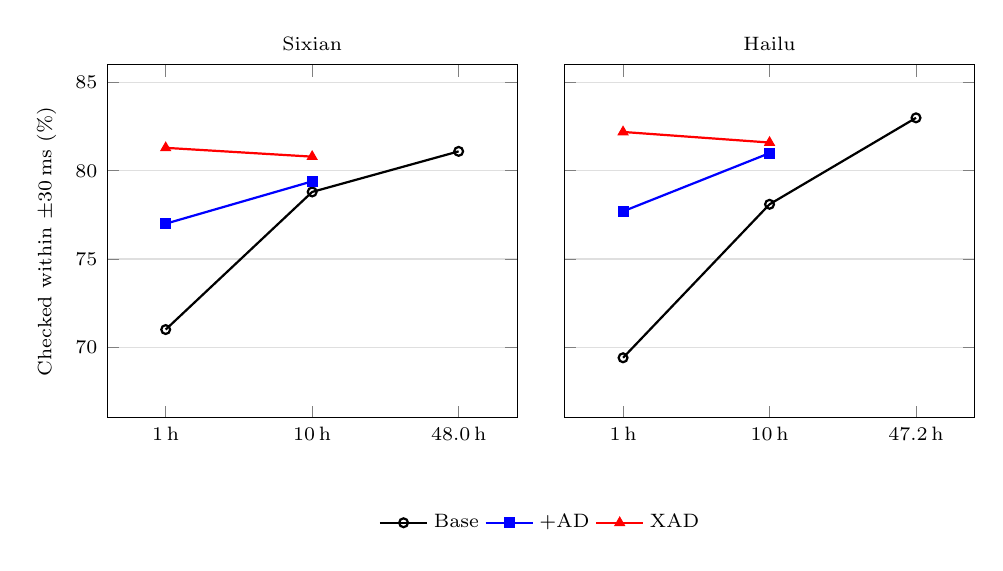
\begin{tikzpicture}
\begin{groupplot}[
  group style={group size=2 by 1, horizontal sep=6mm, y descriptions at=edge left},
  width=0.56\columnwidth, height=0.5\columnwidth,
  xtick=data, enlarge x limits=0.2,
  ymin=66, ymax=86, ytick={70,75,80,85}, ymajorgrids, grid style={gray!25},
  tick label style={font=\scriptsize}, label style={font=\scriptsize}, title style={font=\scriptsize, yshift=-1.5mm},
  legend style={font=\scriptsize, draw=none, fill=none, legend columns=3, at={(1.06,-0.24)}, anchor=north},
  every axis plot/.append style={thick, mark size=1.6pt}]
\nextgroupplot[title=Sixian, symbolic x coords={1\,h,10\,h,48.0\,h}, ylabel={Checked within $\pm$30\,ms (\%)}]
\addplot[black, mark=o] coordinates {(1\,h,71.0) (10\,h,78.8) (48.0\,h,81.1)};
\addplot[blue, mark=square*] coordinates {(1\,h,77.0) (10\,h,79.4)};
\addplot[red, mark=triangle*] coordinates {(1\,h,81.3) (10\,h,80.8)};
\legend{Base, +AD, XAD}
\nextgroupplot[title=Hailu, symbolic x coords={1\,h,10\,h,47.2\,h}]
\addplot[black, mark=o] coordinates {(1\,h,69.4) (10\,h,78.1) (47.2\,h,83.0)};
\addplot[blue, mark=square*] coordinates {(1\,h,77.7) (10\,h,81.0)};
\addplot[red, mark=triangle*] coordinates {(1\,h,82.2) (10\,h,81.6)};
\end{groupplot}
\end{tikzpicture}
\end{document}
